\subsection{Linux sensors}
\begin{figure}[H]
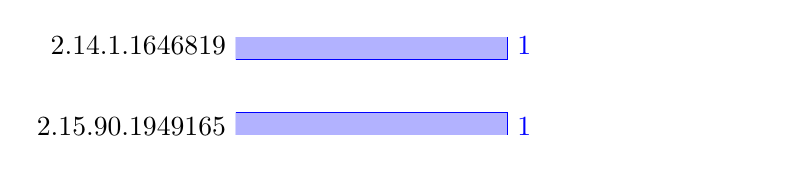
\begin{tikzpicture}
\begin{axis}[
xbar,
y axis line style = { opacity = 0 },
axis x line       = none,
tickwidth         = 0pt,
ytick             = data,
width=0.7\textwidth,
height=80pt,
symbolic y coords = {2.15.90.1949165,2.14.1.1646819,},
nodes near coords
]
\addplot coordinates { (1,2.15.90.1949165) (1,2.14.1.1646819) };
\end{axis}
\end{tikzpicture}
\caption{Linux sensor versions for active devices}
\end{figure}

\subsection{Windows sensors}
\begin{figure}[H]
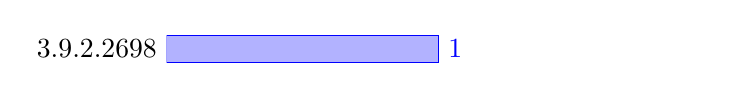
\begin{tikzpicture}
\begin{axis}[
xbar,
y axis line style = { opacity = 0 },
axis x line       = none,
tickwidth         = 0pt,
ytick             = data,
width=0.7\textwidth,
height=60pt,
symbolic y coords = {3.9.2.2698,},
nodes near coords
]
\addplot coordinates { (1,3.9.2.2698) };
\end{axis}
\end{tikzpicture}
\caption{Windows sensor versions for active devices}
\end{figure}

